
% %%%%%%%%%%%%%%%%%%%%%%%%%%%%%%%%%%%%%%%##

% Semester Project Presentation January 2015 at EPFL 

% author: Fabian Brix
% email: fabian.brix@epfl.ch
% École Polytechnique Fédérale de Lausanne, EPFL

% %%%%%%%%%%%%%%%%%%%%%%%%%%%%%%%%%%%%%%%##

\documentclass{beamer}

\usepackage{textpos}
\usepackage{graphicx}
\usepackage{comment}
% for shrinking math symbols
\usepackage{relsize}
\usepackage{booktabs}
\usepackage[normalem]{ulem}
\usepackage[font=footnotesize]{subcaption}

\usepackage{appendixnumberbeamer}

\usetheme{EPFLStyle}

\author{Presentation of Semester Project\\by Fabian Brix}
\title{Energy Load Forecasting}
\subtitle{for the Global Energy Forecasting Competition 2014}
\institute{\ig[width=0.3\paperwidth]{EPFL_LOG_QUADRI_Red.eps}}
%\'Ecole Polytechnique F\'ed\'erale de Lausanne, Switzerland\\


\begin{document} 

\frame{\titlepage}

%%%
\section{Introduction}
\begin{frame}[noframenumbering]{Outline}
\tableofcontents[currentsection]
\end{frame}
\begin{frame}{GEFCom 2014}
\begin{itemize}
%\item GEFCom 2014: 2nd edition of the Global Energy Forecasting Competition
%\pause
\item Dates: 08/15/2014 to 12/15/2014
% \item sponsors: several IEEE bodies and the International Journal of Forecasting
\bigskip
\pause
\item Tracks: energy \textcolor{bostonuniversityred}{load forecasting}, price forecasting, wind, solar
\pause
\item Task: forecast the distribution, in quantiles, of the hourly district load of an energy utility. 
\pause
\item Includes: forecasting the temperature of different zones in the district.
\pause
\item Forecasting horizon: 1 month
\pause
\item Competition type: rolling forecast\\
\pause
$\Rightarrow$ Target for preceding forecasting task published every week to prepare for next horizon
\end{itemize}
\end{frame}


% \section{Motivation}
% \begin{frame}{Personal Motivation}
% \begin{itemize}
% \item Previous attempt at forecasting food commodity prices in Big Data course 
% \pause
% \item $\rightarrow$ Desire to learn about forecasting methodologies
% \end{itemize}
% \end{frame}

%%%
\section{Data}
\begin{frame}[noframenumbering]{Outline}
\tableofcontents[currentsection]
\end{frame}

\begin{frame}{Temperature Data}
\begin{itemize}
\item zonal: 25 series of hourly temperature\\ (Fahrenheit)
\item 01/01/2001 1am to 12/01/2011 midnight.
\end{itemize}
\begin{figure}
\centering
\ig[width=.8\linewidth]{../report/gfx/avg-district-temp-fahrenheit.pdf}
\end{figure}
\end{frame}

\begin{frame}{Load Data}
\begin{itemize}
\item district level: hourly load\\ (Megawatts)
\item 01/01/2005 1am to 12/01/2011 midnight.
\end{itemize}
\begin{figure}
\centering
\ig[width=.8\linewidth]{../report/gfx/utility-load.pdf}
\end{figure}
\end{frame}

%%%
\section{Features}
\begin{frame}[noframenumbering]{Outline}
\tableofcontents[currentsection]
\end{frame}
\begin{frame}{Features}
For temperature \& load:
\begin{itemize}
\item YLAG: $y_{-365 \text{ days}}$
\item DLAG: $y_{-35 \text{ days}}$
\item TOY: time of year
\end{itemize}
\pause
For load only:
\begin{itemize}
\item CTEMP: current temperature
\item DAYT: day type (holiday!)
\end{itemize}
\pause
\begin{table}[h]
\centering
\begin{tabular}{@{}llllllllll@{}}
\toprule
 Type & Mon & Tue & Wed & Thu & Fri & Sat & Sun & \textcolor{bostonuniversityred}{Holiday!} \\ \midrule
SDAYT & 2 & 2 & 2 & 2 & 2 & 1 & 1 & - \\
WDAYT & 2 & 3 & 4 & 5 & 6 & 7 & 1 & - \\
DAYT & 2 & 3 & 4 & 5 & 6 & 7 & 1 & 8 \\ \bottomrule
\end{tabular}
%\caption{Different assignments of integers for days of the week. SDAYT stands for simple day type (weekdays vs. weekends), WDAYT for week day type numbering all days of the week and DAYT includes holidays.}
\end{table}
\end{frame}

%%%
\section{Forecasting Methods}
\begin{frame}[noframenumbering]{Outline}
\tableofcontents[currentsection]
\end{frame}

\begin{frame}{Generalized Additive Model (GAM)}
\begin{itemize}
\item Additive predictor with non-linear functions
\pause
\item $y=s_1(x_1)+s_2(x_2)+\dots+s_p(x_p)+\varepsilon$
\pause
\item $s_i(x_i)$ are smooth functions estimated from the data $x_i$ %(elaborate? formula + splines on extra slide)
\pause
\item Noise $\varepsilon$ assumed to be Gaussian
\pause
\item Use of standard configuration of GAM in R package ``mgcv''
\end{itemize}
%The expected value of the response is a function of a set of predictor variables.
\end{frame}

\begin{frame}{Feedforward Neural Network (NN)}
Configuration using R package nnet
\pause
\begin{itemize}
\item Hidden layer: 1
\pause
\item Hidden units: 5, 10, 15, 20, 25, 30
\pause
\item Linear output for regression
\pause
\end{itemize}
\begin{figure}
\ig<5->[width=.5\linewidth]{gfx/ffnn.pdf}
\end{figure}
\end{frame}

\begin{frame}{Random Forest (RF)}
Configuration using R package randomForest
\pause
\begin{itemize}
\item \# trees: 50, 100, 150, 300
\end{itemize}
\bigskip
\begin{figure}
\ig<3->[width=.5\linewidth]{gfx/rf.png}
\end{figure}
\end{frame}

\begin{frame}{Forecasting Models}
\begin{itemize}
\item Model: hyperparameter settings + formula 
\pause
\item Formula: collection of features used in model (R)\\
\pause
$\Rightarrow$ Create point forecasts with different forecasting methods
\end{itemize}
\end{frame}

%%%
\section{Quantile Forecasting}
\begin{frame}[noframenumbering]{Outline}
\tableofcontents[currentsection]
\end{frame}
\begin{frame}{Quantile Forecasting}
%http://robjhyndman.com/hyndsight/quantile-forecasts-in-r/

%Required are Percentile Forecasts. 
%Quantile: Upper bound value of forecasts with cumulative probability $\tau$, $q_\tau$.
\begin{itemize}
\item Future: random variable with ``forecast distribution''
\pause
\item ``Quantile forecast'': quantiles of this distribution (percentiles)
\pause
\item Point forecasts correspond to mean of forecast distribution\\
\pause
$\rightarrow$ Offset \textcolor{bostonuniversityred}{quantiles of training residuals} by point forecast
\end{itemize}
%http://www.lokad.com/quantile-regression-(time-series)-definition!

\begin{figure}
\ig<6->[width=.7\linewidth]{gfx/quantile-forecast.pdf}
\end{figure}
%\begin{columns}[c]
%\column{.49\framewidth}
%include graphic with point forecast here
%\column{.49\framewidth}
%\end{columns}

%The future value of a time series is unknown, so you can think of it as a ran­dom vari­able, and its dis­tri­b­u­tion is the “fore­cast dis­tri­b­u­tion”. A “quan­tile fore­cast” is a quan­tile of the fore­cast dis­tri­b­u­tion. The usual point fore­cast is often the mean or the median of the fore­cast dis­tri­b­u­tion.

%A pre­dic­tion inter­val is a range of spec­i­fied cov­er­age prob­a­bil­ity under that dis­tri­b­u­tion. For exam­ple, if we assume the fore­cast dis­tri­b­u­tion is nor­mal, then the 95\% pre­dic­tion inter­val is defined by the 2.5\% and 97.5\% quan­tiles of the fore­cast distribution
\end{frame}

%%%
\section{Error Measures}
\begin{frame}[noframenumbering]{Outline}
\tableofcontents[currentsection]
\end{frame}

\begin{frame}{Mean Average Percentage Error}
\begin{itemize}
\item Used to evaluate goodness of fit
\pause
\item Scale-independent (\%)
\end{itemize}
\pause
\[
\text{MAPE}=\frac{100}{N}\sum^N_{i=1} \left|\frac{\xi_i}{y_i}\right|
\]
\pause
\begin{itemize}
\item $\text{residual:}\quad \xi_i=y_i - \hat{y}_i$
\pause
\item $y_i$: time series value at time $i$
\item $\hat{y}_i$: forecast at time $i$
\end{itemize}
\end{frame}

\begin{frame}{Pinball Loss Function}
%Generalization of mean absolute error for quantile forecasts
%It can be proved that the function that minimizes the pinball loss delivers the optimal quantile as well
%Slope reflects the desired imbalance in the quantile forecast
\begin{itemize}
\item Used to evaluate quantile forecasts
\item And measure performance against competition leaderboard
\pause
\item Strictly positive, the lower the more accurate the forecast
\pause
\item Score at $i$ given by $\text{mean}(L_{0.01}, L_{0.02}, \dots, L_{0.99})$
\end{itemize}
\pause
\[
  L_{\tau}(\xi)=\begin{cases} \tau \xi & \text{if } \xi \geq 0 \\
                                          (\tau-1)\xi & \text{if } \xi < 0 
                                  \end{cases} \quad\text{where } \xi=(y_i-\hat{y}_{i,\tau})
\]

\begin{figure}
\centering
\ig<4->[width=.8\linewidth]{gfx/pinball.pdf}
\end{figure}
%The pinball loss function (in red) has been named after its shape that looks like the trajectory of a ball on a pinball. 
%the further away from the target y, the larger the value of Lτ(y,z).
%The slope is used to reflect the desired imbalance in the quantile forecast.
\end{frame}

%\subsection{Time series cross-validation}
\section{Method Evaluation}
\begin{frame}[noframenumbering]{Outline}
\tableofcontents[currentsection]
\end{frame}
\begin{frame}{Method Evaluation}
\begin{itemize}
\item Use whole competition dataset 
\pause
\item Initial data + 14 months from subsequent tasks
\pause
\item Use rolling forecast of 14 month period to evaluate forecasts
\end{itemize}
\pause
\begin{figure}
\centering
\ig<3>[width=.9\linewidth]{gfx/cross-correlation-1.pdf}
\ig<4>[width=.9\linewidth]{gfx/cross-correlation-2.pdf}
\ig<5>[width=.9\linewidth]{gfx/cross-correlation-3.pdf}
\end{figure}

%After creating the features for the whole dataset, we run through the whole dataset, temperature and load respectively, in a rolling fashion to create our predictions. This approach can be described as ``forecast evaluation with a rolling origin''. However, since, according to Hyndman \cite{Rob}, it is the natural and obvious analogue to leave-one-out cross-validation for cross-sectional data origins, we can call it ``time series cross-validation''.\par
\end{frame}


%%%



\begin{frame}{Workflow Diagram}
\begin{figure}
\centering
\hspace*{-1.5em}
\ig[width=1.1\linewidth]{gfx/workflow.pdf}
\end{figure}
\end{frame}

%%%
\section{Results}
\begin{frame}[noframenumbering]{Outline}
\tableofcontents[currentsection]
\end{frame}
\begin{frame}{Results - Temperature}
\begin{itemize}
\item Best score: 12.04\% MAPE
\pause
\item Model: neural network and 30 hidden units
\end{itemize}
\begin{columns}[c] % the "c" option specifies center vertical alignment
    \column{.5\textwidth} % column designated by a command
        \begin{figure}
		\centering
		\ig<3->[width=.8\textwidth]{gfx/NN-temp-plot.pdf}
		\end{figure}
    \column{.5\textwidth}
	    \begin{figure}
		\centering
		\hspace*{-3em}
		\ig<4->[width=1.3\textwidth]{../report/gfx/results/temp/TEMP-MONTHLY-BEST-COLUMNS.pdf}
		\end{figure}
\end{columns}
\end{frame}


\begin{frame}{Results - Load}
\begin{itemize}
\item Effect of temperature\\
$\rightarrow$ Significant: -2.5\% MAPE
\pause
\item No effect of different temperature preprocessing (average, PCA, 1 series)
\pause
\item Predicting temperature for training period of load forecast\\
$\rightarrow$ Pinball error improves
\pause
\item Effect of forecast horizon\\
$\rightarrow$ results improved with 1 week horizon % exploiting more recent lags
\pause
\item Effect of daytypes\\
$\rightarrow$ better results without
\end{itemize}
\end{frame}

\begin{frame}{Best Configuration}
\begin{itemize}
\item Random forest, 100 trees, 1 week f. horizon 
%\item Neural Network, 15 hidden networks, 1 month f. horizon %forecasting horizon: 1month)
%\item Temperature prediction for load training period
%\item \sout{Daytype}
\pause
\item MAPE: 16.1\%, Pinball: 7.999 
 %11 tasks, Excluding the first three months (Oct, Nov, Dec) that were the trial period and the last month for which the real data has not been published
\end{itemize}
\begin{columns}[c] % the "c" option specifies center vertical alignment
    \column{.5\textwidth} % column designated by a command
        \begin{figure}
		\centering
		\ig<3->[width=.65\textwidth]{gfx/RF-load-plot.pdf}
		\end{figure}
    \column{.5\textwidth}
	    \begin{figure}
		\centering
		\hspace*{-1.8em}
		\ig<4->[width=1.2\textwidth]{../report/gfx/results/load/LOAD-BEST-PINBALL.pdf}
		\end{figure}
\end{columns}

\end{frame}
%Using the pinball errors displayed in figure 16a we can now compute a hypothetical position on the
%The participants are required to submit entries for at least 9 out of 12 weeks during the scoring period to be eligible for a position in the final leaderboard.”
%The positions on the scoreboards for the individual tasks are displayed in figure 16b comparing the different prediction horizons. 
%The average position for the task leaderboards would be 5.64. However, not every contestant reached a position equally high up the scoreboard every week allowing for our improved hypothetical position on the final leaderboard.

\begin{frame}{Best Configuration - Final Leaderboard}
\begin{itemize}
\item Trimmed pinball mean: 7.16 $\Rightarrow$ \#3 %(discarding best \& worst score):\\
%$\rightarrow$ 7.16 (\#3, 6.93, 7.10)
\item Average position on task leaderboards: 5.64
\item Not every contestant reaches equally high scores every week
\end{itemize}

\begin{figure}
\centering
\ig[width=.6\linewidth]{../report/gfx/results/load/LOAD-BEST-POSITION.pdf}
\end{figure}
\end{frame}

\begin{frame}{Further Work}
\begin{itemize}
\item Find a development environment which makes debugging easier (R in vim)
\pause
\item Analyze training residuals \pause $\rightarrow$ white noise
\pause
\item Further research on random forests for regression
\pause
\item Produce and evalute ensemble forecasts
\end{itemize}
\end{frame}
%\begin{frame}[noframenumbering]
%\centering
%Thank you for your attention!
%\end{frame}

% All your regular slides
% After your last numbered slide
\appendix
\newcounter{finalframe}
\setcounter{finalframe}{\value{framenumber}}
% Backup frames
\setcounter{framenumber}{\value{finalframe}}


%%%%%%%%%%
%APPENDIX%
%%%%%%%%%%
\begin{frame}{Forecasting Horizon - Trick}
\begin{itemize}
\item Forecasts with two different time horizons: 1 month vs 1 week
\item Forecasts of week 1 to 4 are combined + rest of monthly forecast 
\end{itemize}
%The idea behind the weekly forecasts is to allow for shorter, but increasing time lags in week 1, 2, 3 and 4 of the month constituting the time horizon. The forecasts of week 1 to 4 are then combined with the rest of the forecast from the monthly forecasts.
%temperature vs load!
\begin{figure}
\centering
\hspace*{-1.5em}
\ig[width=1.1\linewidth]{gfx/forecasting-horizon.pdf}
\end{figure}
\end{frame}

\begin{frame}{Features}
\begin{figure}[!ht]
\centering
\begin{subfigure}[b]{.4\linewidth}
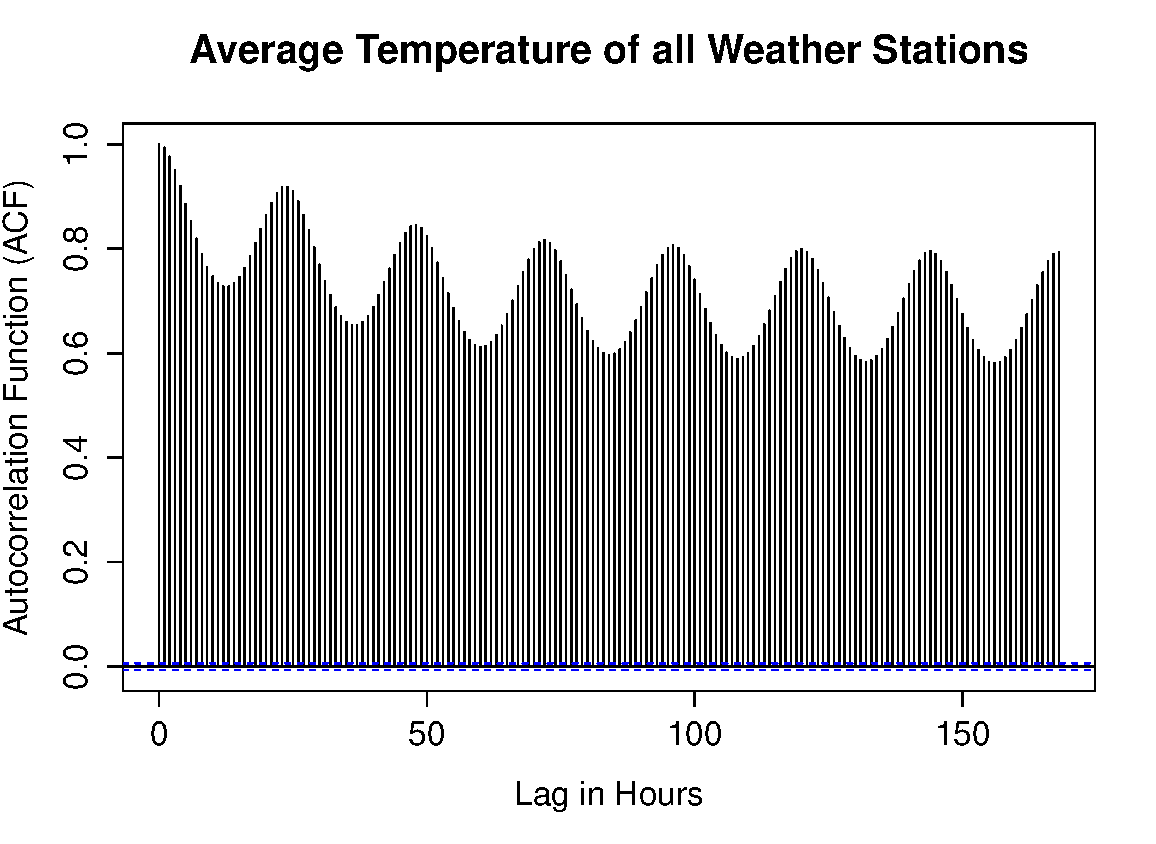
\includegraphics[width=\linewidth]{../report/gfx/acf_avg_temp_7days.pdf}
\caption{time lag: 7 days, 168 hours}
\label{subfig:avg-temp-7days}
\end{subfigure}
\begin{subfigure}[b]{.4\linewidth}
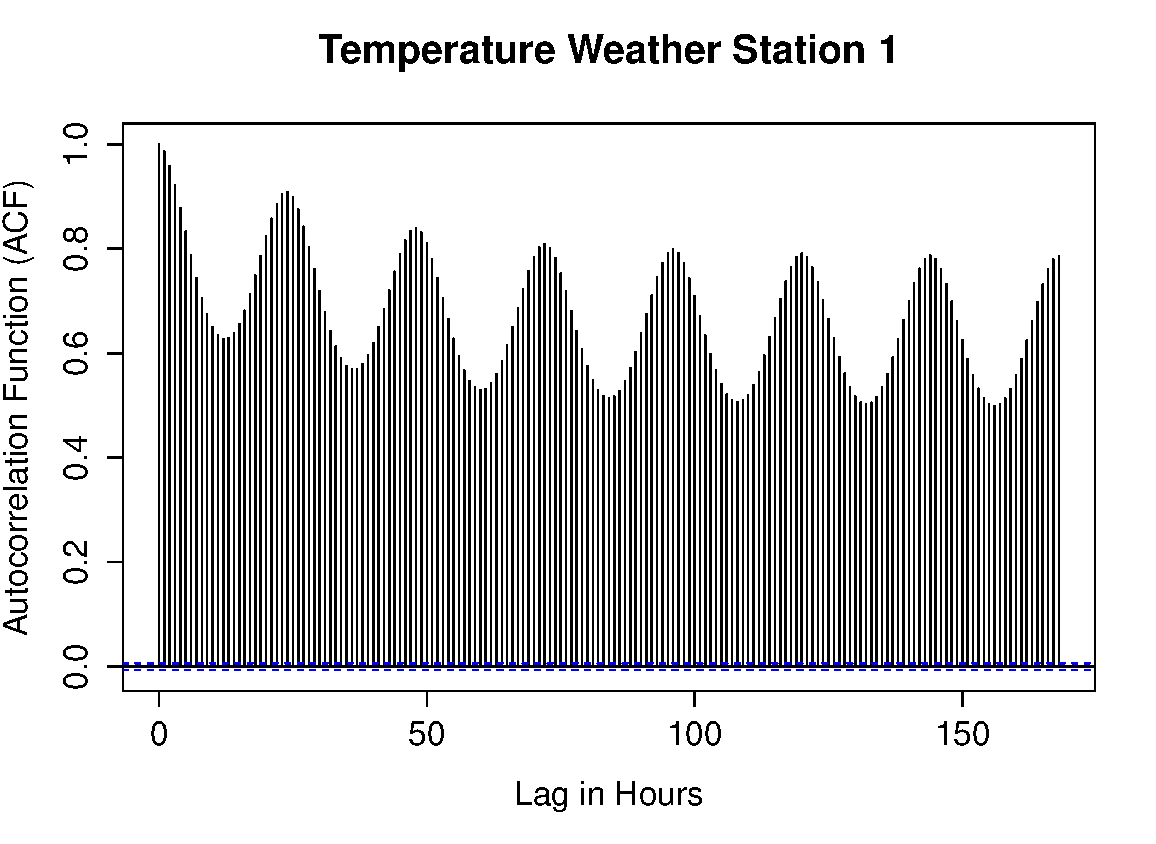
\includegraphics[width=\linewidth]{../report/gfx/acf_temp_station1_7days.pdf}
\caption{time lag: 7 days, 168 hours}
\label{subfig:temp-station1-7days}
\end{subfigure}

\begin{subfigure}[b]{.4\linewidth}
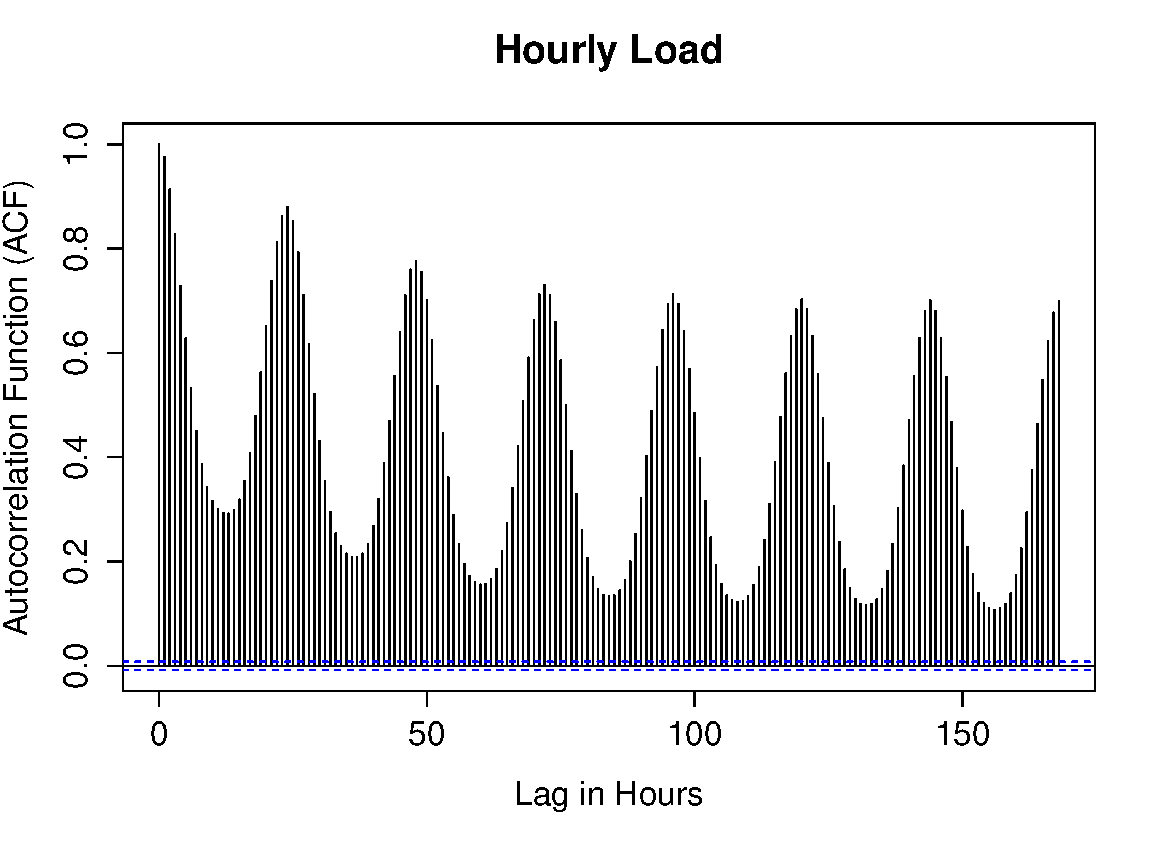
\includegraphics[width=\linewidth]{../report/gfx/acf-load-7days.pdf}
\caption{lag: 7 days, 168 hours}
\label{subfig:acf-load-7days}
\end{subfigure}
\begin{subfigure}[b]{.4\linewidth}
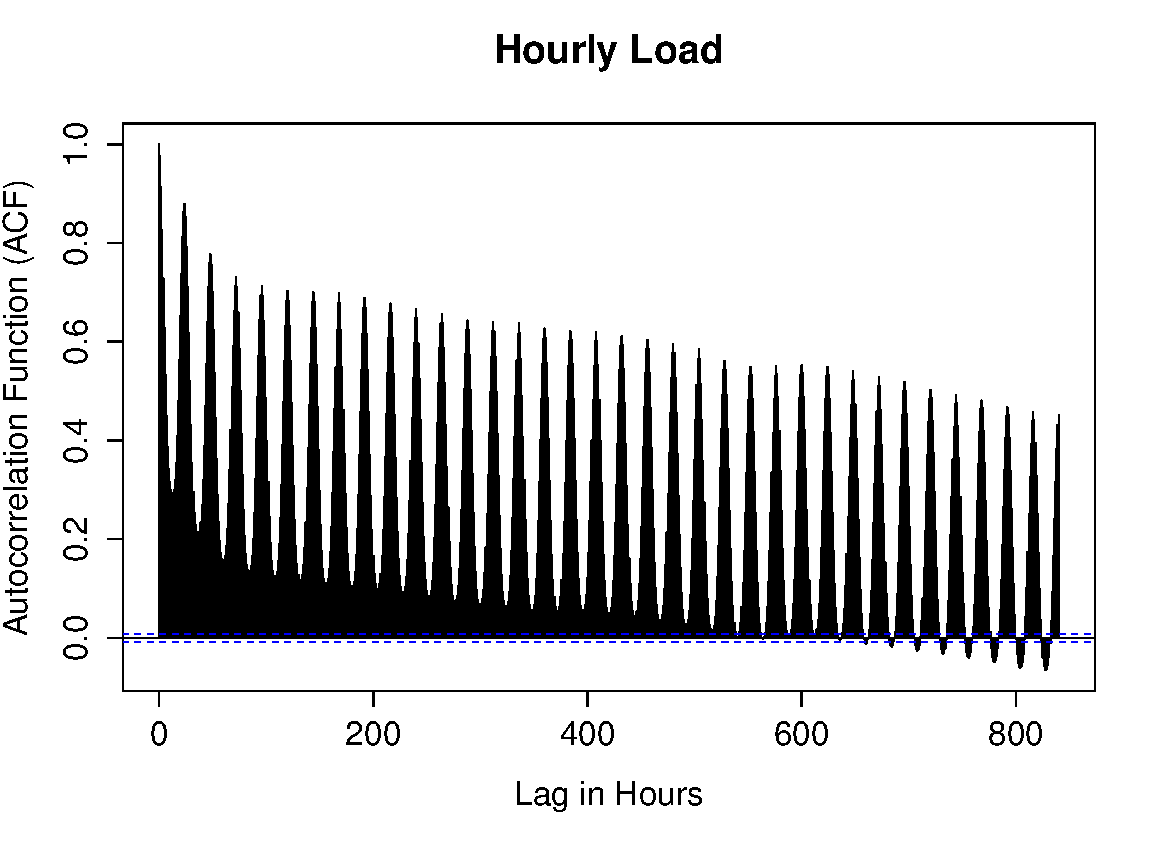
\includegraphics[width=\linewidth]{../report/gfx/acf-load-35days.pdf}
\caption{lag: 35 days, 840 hours}
\label{subfig:acf-load-35days}
\end{subfigure}
\label{fig:acf-load}
\end{figure}
\end{frame}

% \begin{frame}{GAM - Splines}
% \end{frame}

\begin{frame}{Residual Plot}
\begin{figure}
\centering
\ig[width=.7\linewidth]{gfx/Winning-Conf-Res-Plot.pdf}
\end{figure}
%TODO! using blog entry
%http://blog.minitab.com/blog/adventures-in-statistics/why-you-need-to-check-your-residual-plots-for-regression-analysis
\end{frame}

% \begin{frame}{GAM - Splines}
% \begin{figure}
% \centering
% \ig[width=.7\linewidth]{gfx/Winning-Conf-Res-Plot.pdf}
% \end{figure}
% %TODO! using blog entry
% %http://blog.minitab.com/blog/adventures-in-statistics/why-you-need-to-check-your-residual-plots-for-regression-analysis
% \end{frame}
% \begin{frame}{Residuals}
% \end{frame}

% \begin{frame}{Decision Trees}
% \end{frame}
\end{document} 